% !TEX root = main.tex

%%%%%%%%%%%%%%%%%%%%%%%%%%%%%%%%%%%%%%%%%%%%%%%%%%%%%%%%%%%%%%%%%%%%%%%%%%%%%%%%%%%%%%%%%%%%%%%%
\section{結果}
%%%%%%%%%%%%%%%%%%%%%%%%%%%%%%%%%%%%%%%%%%%%%%%%%%%%%%%%%%%%%%%%%%%%%%%%%%%%%%%%%%%%%%%%%%%%%%%%

\subsection{実験課題1}
ソレノイド底面を$z=0\,[\si{cm}]$とし,各$z$座標における測定結果を以下の
図5~図25に示す.また,$z$座標と磁気プローブの出力$V_{co}$の積分である
$\int_{0}^{t}V_{co}(t)dt$との測定結果を表1に示す.
ただし,磁気プローブの出力$V_{co}$の積分はオシロスコープから得られるデジタルデータ
(テキストデータ)を使用して算出する方法を用いる.

\begin{figure}[H]
    \centering
    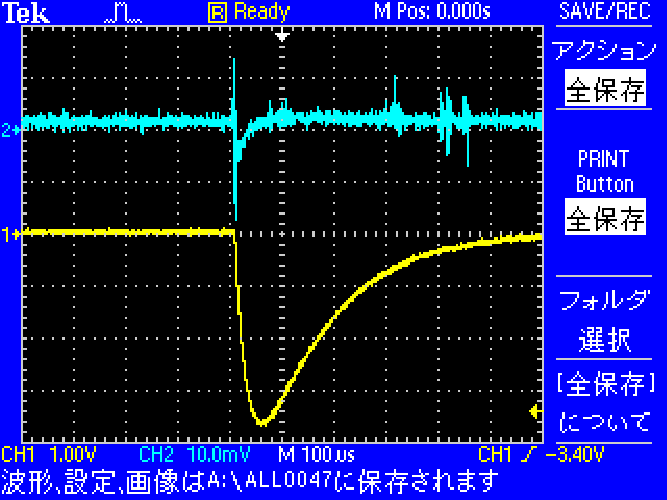
\includegraphics[scale=0.5]{images-22.pdf}
    \caption{$z=-8\,[cm]$における測定結果}
\end{figure}

\begin{figure}[H]
    \centering
    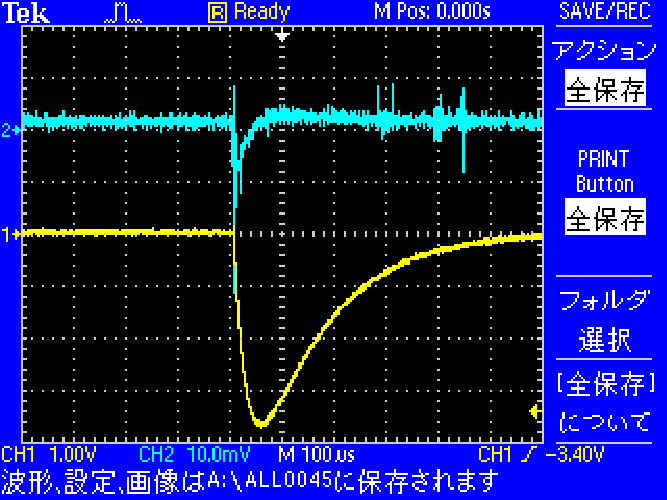
\includegraphics[scale=0.5]{images-21.pdf}
    \caption{$z=-6\,[cm]$における測定結果}
\end{figure}

\begin{figure}[H]
    \centering
    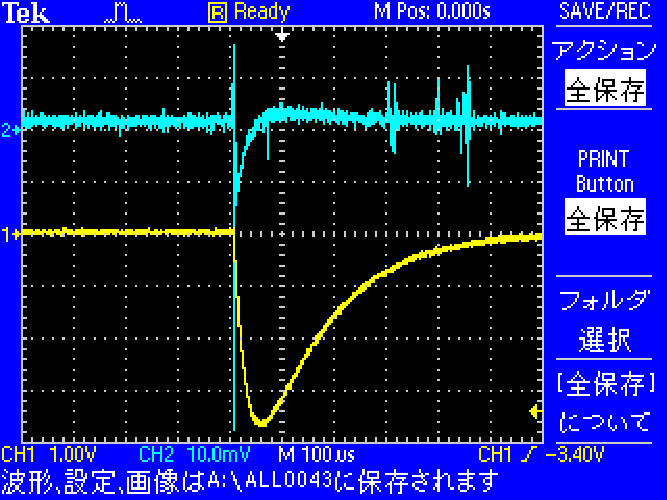
\includegraphics[scale=0.5]{images-20.pdf}
    \caption{$z=-4\,[cm]$における測定結果}
\end{figure}

\begin{figure}[H]
    \centering
    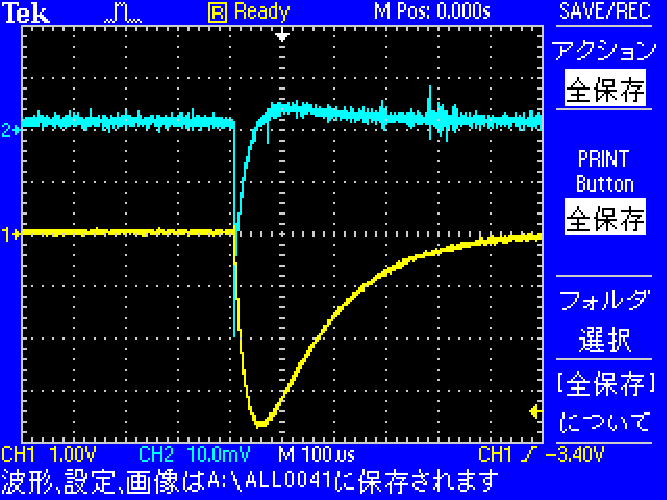
\includegraphics[scale=0.5]{images-19.pdf}
    \caption{$z=-2\,[cm]$における測定結果}
\end{figure}

\begin{figure}[H]
    \centering
    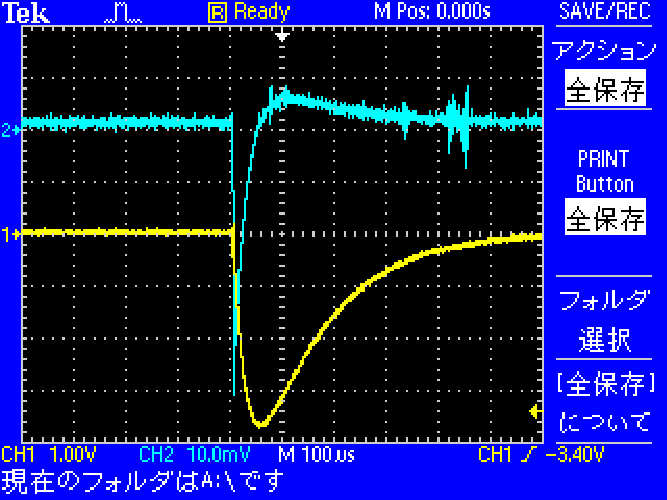
\includegraphics[scale=0.5]{images-1.pdf}
    \caption{$z=0\,[cm]$における測定結果}
\end{figure}

\begin{figure}[H]
    \centering
    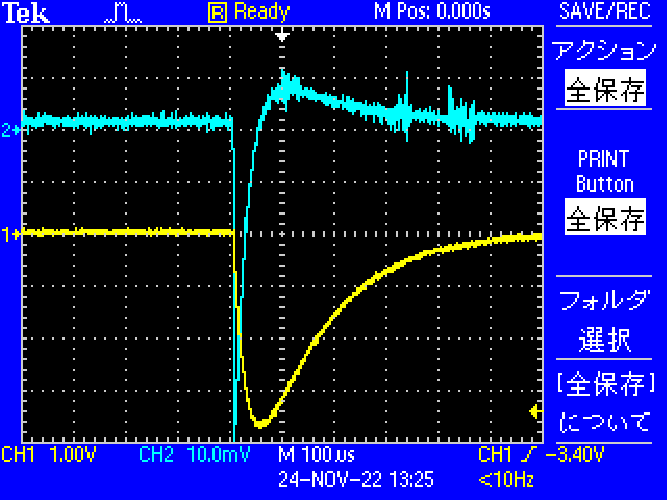
\includegraphics[scale=0.5]{images-2.pdf}
    \caption{$z=2\,[cm]$における測定結果}
\end{figure}

\begin{figure}[H]
    \centering
    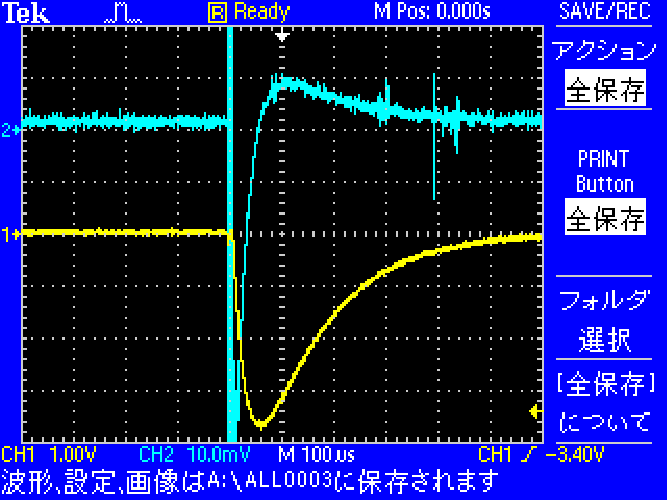
\includegraphics[scale=0.5]{images-3.pdf}
    \caption{$z=4\,[cm]$における測定結果}
\end{figure}

\begin{figure}[H]
    \centering
    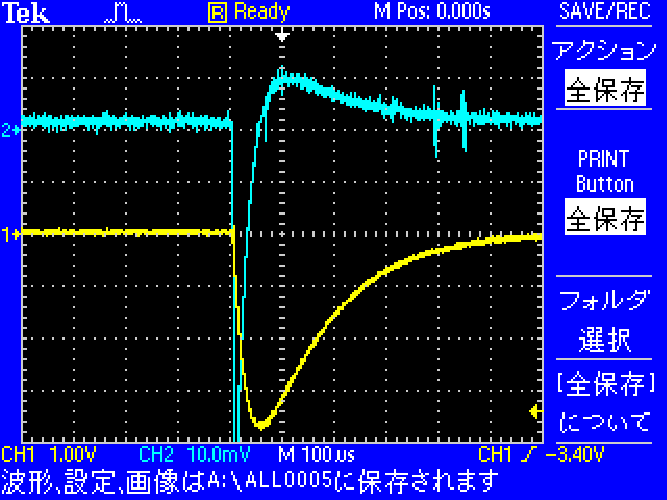
\includegraphics[scale=0.5]{images-4.pdf}
    \caption{$z=6\,[cm]$における測定結果}
\end{figure}

\begin{figure}[H]
    \centering
    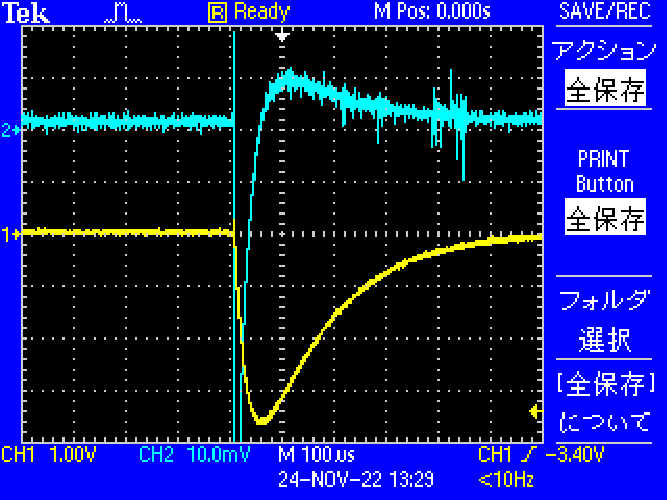
\includegraphics[scale=0.5]{images-5.pdf}
    \caption{$z=8\,[cm]$における測定結果}
\end{figure}

\begin{figure}[H]
    \centering
    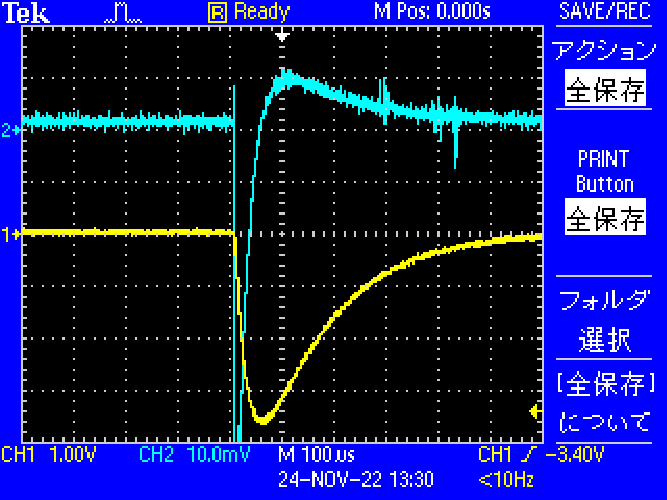
\includegraphics[scale=0.5]{images-6.pdf}
    \caption{$z=10\,[cm]$における測定結果}
\end{figure}

\begin{figure}[H]
    \centering
    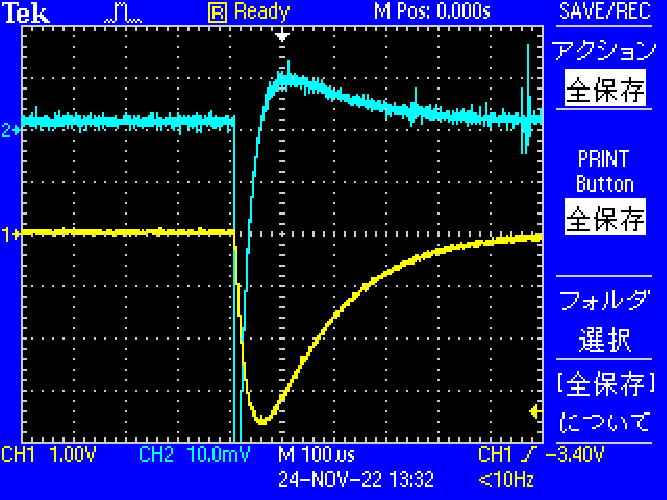
\includegraphics[scale=0.5]{images-7.pdf}
    \caption{$z=12\,[cm]$における測定結果}
\end{figure}

\begin{figure}[H]
    \centering
    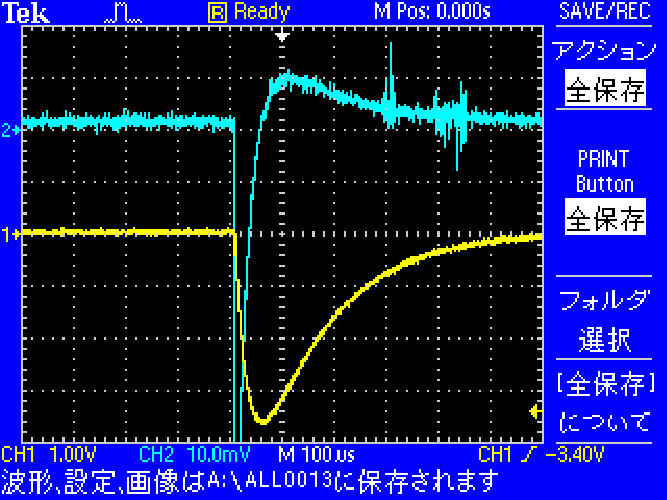
\includegraphics[scale=0.5]{images-8.pdf}
    \caption{$z=14\,[cm]$における測定結果}
\end{figure}

\begin{figure}[H]
    \centering
    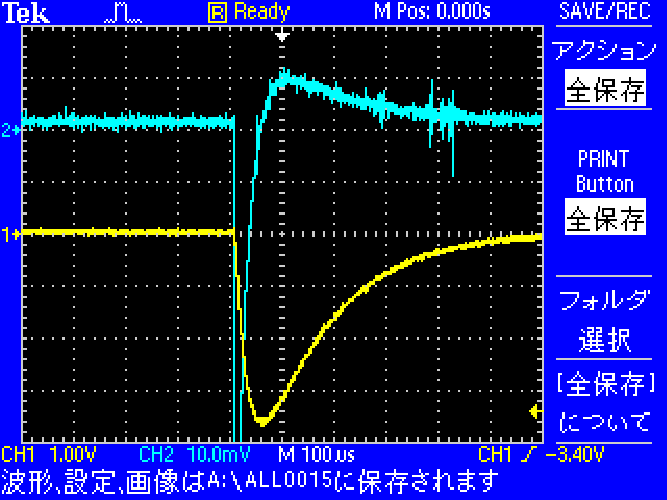
\includegraphics[scale=0.5]{images-9.pdf}
    \caption{$z=16\,[cm]$における測定結果}
\end{figure}

\begin{figure}[H]
    \centering
    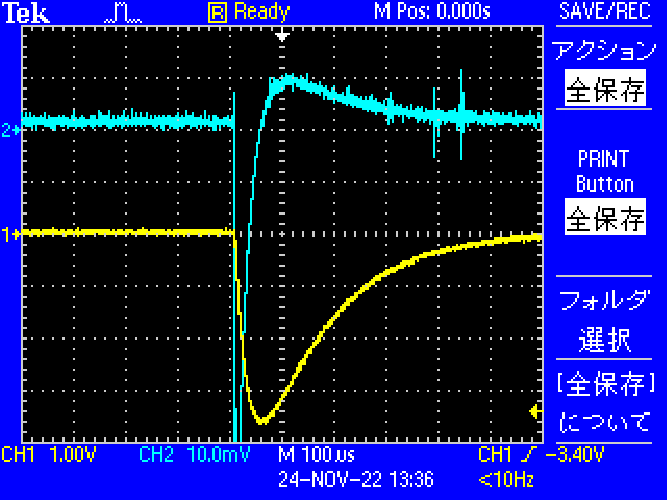
\includegraphics[scale=0.5]{images-10.pdf}
    \caption{$z=18\,[cm]$における測定結果}
\end{figure}

\begin{figure}[H]
    \centering
    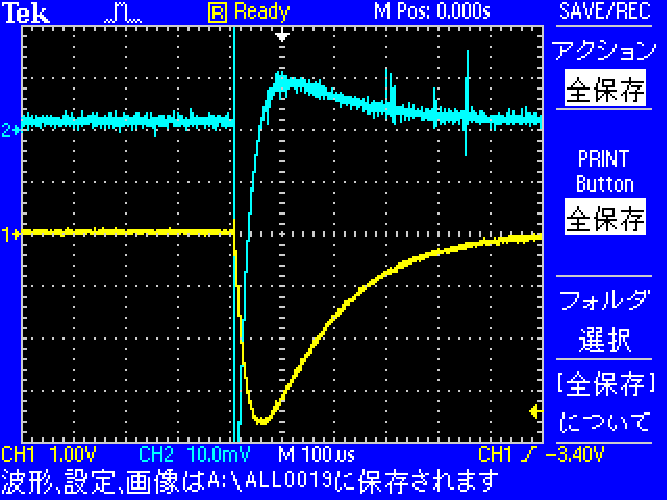
\includegraphics[scale=0.5]{images-11.pdf}
    \caption{$z=20\,[cm]$における測定結果}
\end{figure}

\begin{figure}[H]
    \centering
    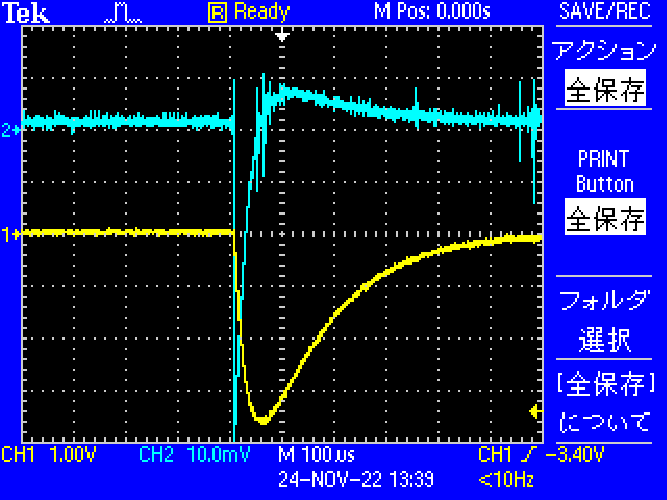
\includegraphics[scale=0.5]{images-12.pdf}
    \caption{$z=22\,[cm]$における測定結果}
\end{figure}

\begin{figure}[H]
    \centering
    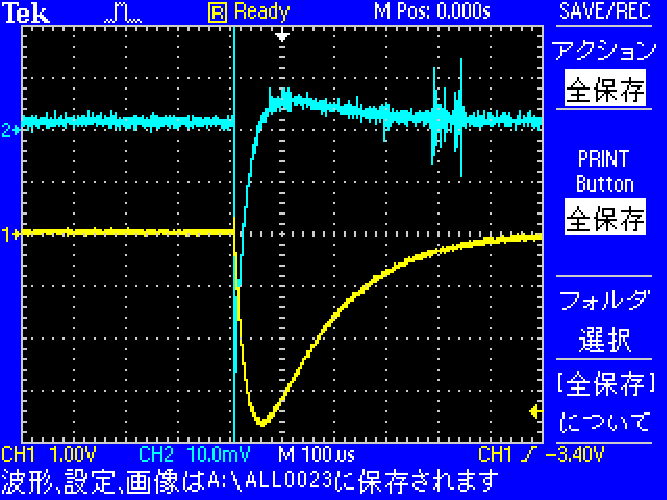
\includegraphics[scale=0.5]{images-13.pdf}
    \caption{$z=24\,[cm]$における測定結果}
\end{figure}

\begin{figure}[H]
    \centering
    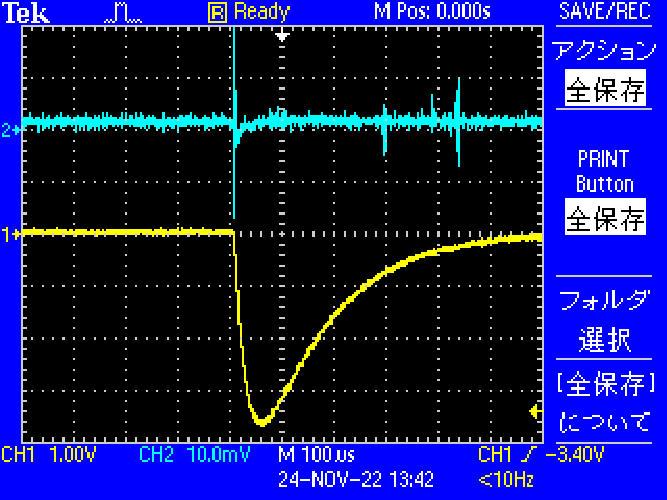
\includegraphics[scale=0.5]{images-14.pdf}
    \caption{$z=26\,[cm]$における測定結果}
\end{figure}

\begin{figure}[H]
    \centering
    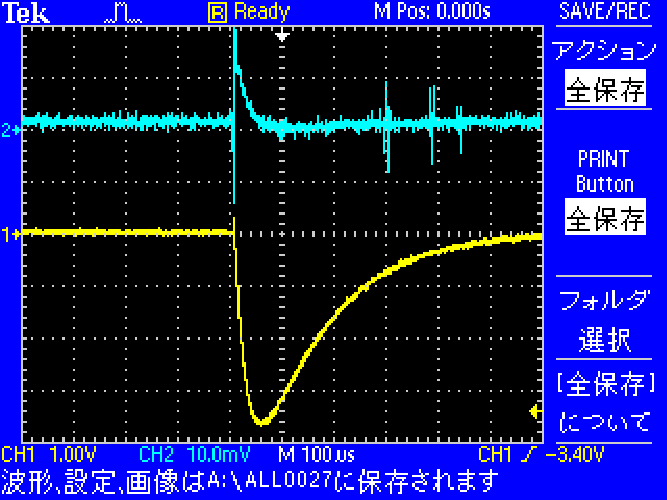
\includegraphics[scale=0.5]{images-15.pdf}
    \caption{$z=28\,[cm]$における測定結果}
\end{figure}

\begin{figure}[H]
    \centering
    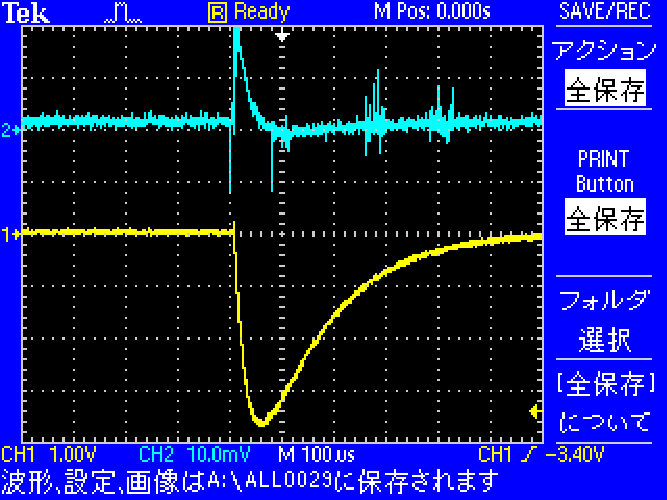
\includegraphics[scale=0.5]{images-16.pdf}
    \caption{$z=30\,[cm]$における測定結果}
\end{figure}

\begin{figure}[H]
    \centering
    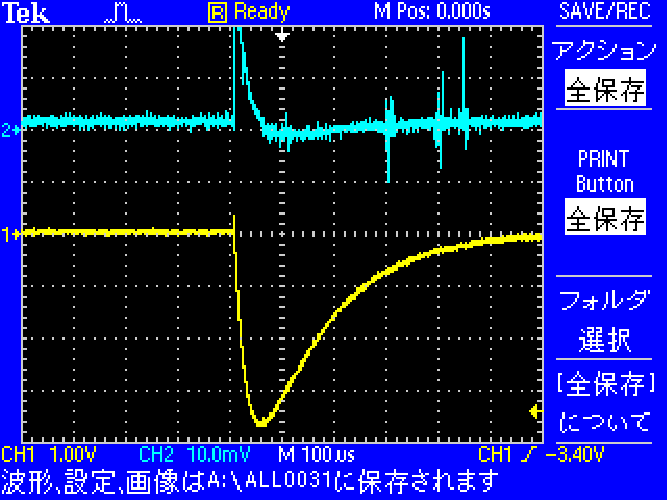
\includegraphics[scale=0.5]{images-17.pdf}
    \caption{$z=32\,[cm]$における測定結果}
\end{figure}

\begin{table}[H]
    \centering
    \caption{磁気プローブの出力$V_{co}$の積分結果}
    \begin{tabular}{c|c}
    \hline
        $z座標\,[\si{cm}]$ & $\int_{0}^{t}V_{co}(t)dt\,[\si{\mu\volt}]$ \\ \hline
        -8 & 0.0706 \\ 
        -6 & 0.154 \\ 
        -4 & 0.221 \\ 
        -2 & 0.421 \\ 
        0 & 0.794 \\ 
        2 & 1.14 \\ 
        4 & 1.40 \\ 
        6 & 1.46 \\ 
        8 & 1.47 \\ 
        10 & 1.49 \\ 
        12 & 1.51 \\ 
        14 & 1.51 \\ 
        16 & 1.49 \\ 
        18 & 1.46 \\ 
        20 & 1.39 \\ 
        22 & 1.04 \\ 
        24 & 0.768 \\ 
        26 & 0.394 \\ 
        28 & 0.336 \\ 
        30 & 0.511 \\ 
        32 & 0.591 \\ \hline
    \end{tabular}
\end{table}

\newpage

\subsection{実験課題2}
鎖交数を変化させた際の,各鎖交数における測定結果を図26~図30に示す.
また,鎖交数と,抵抗$R$の両端の電圧波形$V_R$のピーク電圧$V_{Rmax}$と,
ロゴスキーコイルの出力$V_e$の積分である$\int_{0}^{t}V_e(t)dt$
との測定結果を表2に示す.ただし,ロゴスキーコイルの出力$V_e$の積分は
オシロスコープから得られるデジタルデータ
(テキストデータ)を使用して算出する方法を用いる.

\begin{figure}[H]
    \centering
    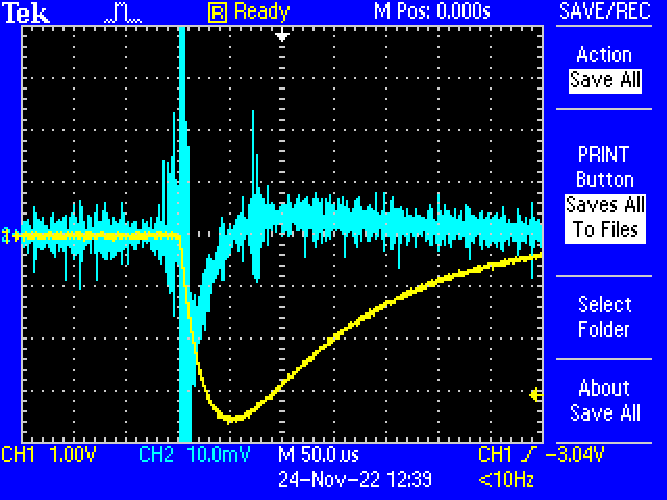
\includegraphics[scale=0.5]{rogowskii-1.pdf}
    \caption{鎖交数が1の時の測定結果}
\end{figure}

\begin{figure}[H]
    \centering
    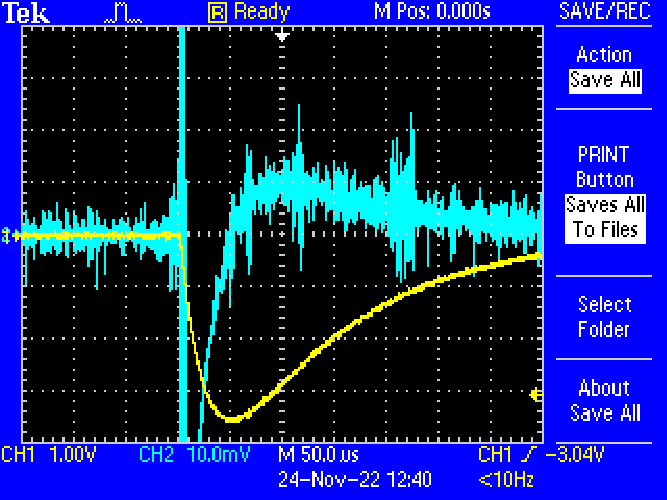
\includegraphics[scale=0.5]{rogowskii-2.pdf}
    \caption{鎖交数が2の時の測定結果}
\end{figure}

\begin{figure}[H]
    \centering
    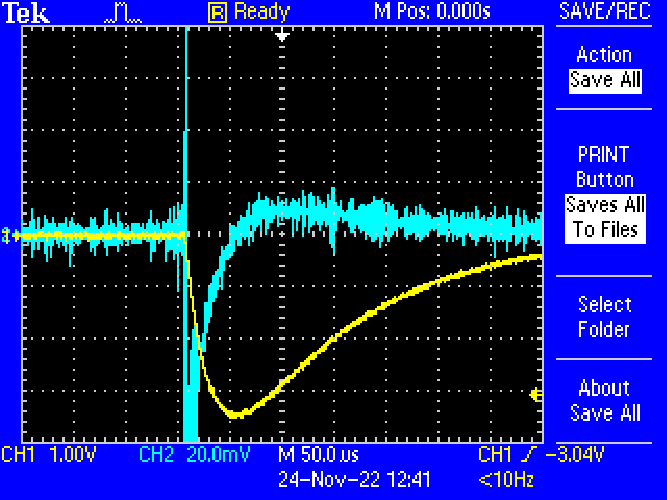
\includegraphics[scale=0.5]{rogowskii-3.pdf}
    \caption{鎖交数が3の時の測定結果}
\end{figure}

\begin{figure}[H]
    \centering
    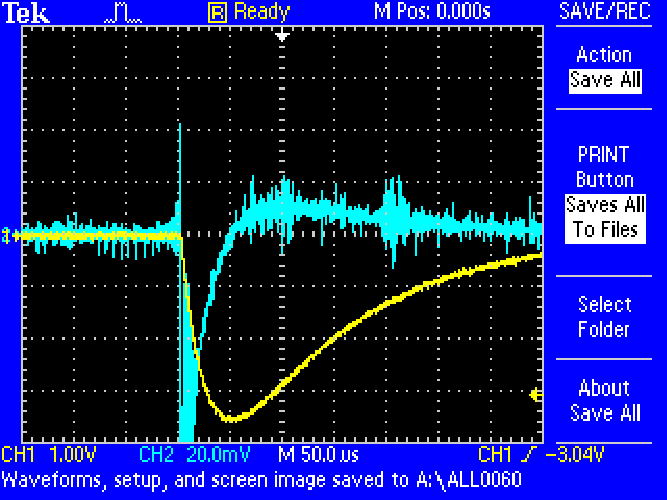
\includegraphics[scale=0.5]{rogowskii-4.pdf}
    \caption{鎖交数が4の時の測定結果}
\end{figure}

\begin{figure}[H]
    \centering
    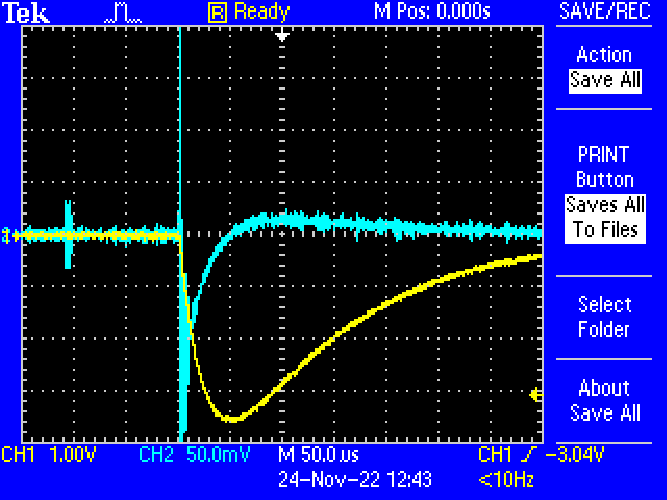
\includegraphics[scale=0.5]{rogowskii-5.pdf}
    \caption{鎖交数が5の時の測定結果}
\end{figure}

\begin{table}[!ht]
    \centering
    \caption{ロゴスキーコイルの出力$V_e$の積分結果}
    \begin{tabular}{c|c}
    \hline
        鎖交回数 & $\int_{0}^{t}V_e(t)dt\,[\si{\mu \volt}]$ \\ \hline
        1 & 0.523 \\ 
        2 & 1.09 \\ 
        3 & 1.53 \\ 
        4 & 1.70 \\ 
        5 & 2.39 \\ \hline
    \end{tabular}
\end{table}